\documentclass{standalone}
\usepackage{tikz}
\begin{document}
\begin{centering}
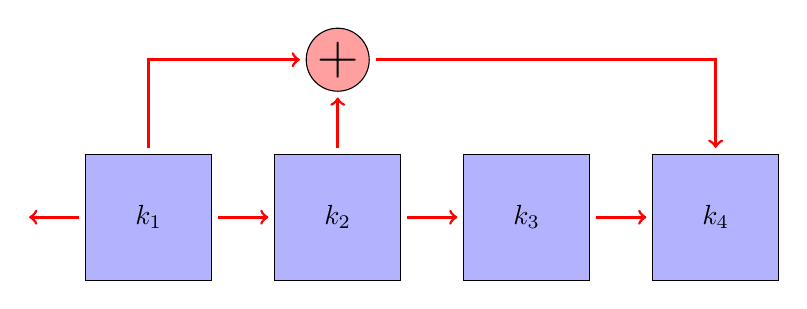
\begin{tikzpicture} [scale = 0.8]
	\draw[line width=1, color=red, <-] (-6.9,1) -- (-6.1,1);
	\fill[blue!30] (-6,0) rectangle (-4,2);
	\draw[thin] (-6,0) rectangle (-4,2);
	\node at (-5,1) {$k_1$} ;
	\draw[line width=1, color=red, ->] (-3.9,1) -- (-3.1,1);
	\fill[blue!30] (-3,0) rectangle (-1,2);
	\draw[thin] (-3,0) rectangle (-1,2);
	\node at (-2,1) {$k_2$} ;
	\draw[line width=1, color=red, ->] (-0.9,1) -- (-0.1,1);
	\fill[blue!30] (0,0) rectangle (2,2);
	\draw[thin] (0,0) rectangle (2,2);
	\node at (1,1) {$k_3$} ;
	\draw[line width=1, color=red, ->] (2.1,1) -- (2.9,1);
    \fill[blue!30] (3,0) rectangle (5,2);
    \draw[thin] (3,0) rectangle (5,2);
    \node at (4,1) {$k_4$} ;
	\draw [fill = pink!150] (-2,3.5) circle [radius = 0.5] node {\huge $+$};
	\draw [line width=1, color = red, ->] (-2,2.1) -- (-2, 2.9);
	\draw [line width=1, color = red, ->] (-5,2.1) -- (-5, 3.5) -- (-2.6,3.5);
	\draw [line width=1, color = red, ->] (-1.4,3.5) -- (4, 3.5) -- (4,2.1);
\end{tikzpicture}
\end{centering}
\end{document}
